%%=====================================================================
%\chapter{Abstract Language  for Description of Interactive Message}
%\label{aladim}
%%=====================================================================
%
%A  \aladim\ ({\em \Aladim})  é uma  linguagem de  modelagem construída
%para       atender       aos       requisitos      enumerados       no
%capítulo~\ref{introduction}. Ela possui alguns conceitos cujas origens
%remontam   a    linguagem   \imml\   ({\em   \Imml})~\cite{Leite:2003,
%  CostaNeto:2005,CostaNeto:Leite:2006},   e,   como   tal,  também   é
%concebida  com  base na  \se~\cite{deSouza:2005}.   Na \imml,  segundo
%\citeonline{Leite:2005}, a  interface de usuário  deve {\em comunicar}
%ao  usuário as  respostas a  duas questões  fundamentais:  (i) ``quais
%tipos   de  problemas   que   essa  aplicação   está  preparada   para
%solucionar?''  (que corresponde às funcionalidades da aplicação); (ii)
%``como estes  problemas podem  ser resolvidos?''  (que  corresponde ao
%processo de interação da aplicação).
%
%Em  linhas gerais,  este trabalho  considera  que o  {\em processo  de
%  interação} ocorre quando o usuário  entra em contato sensorial com a
%interface de um  {\em sistema interativo}, com o  objetivo de usufruir
%de  determinadas  {\em  funcionalidades}  oferecidas  pela  aplicação.
%Nesse processo, a comunicação aflora de maneira que o sistema, através
%da sua interface, revela ao usuário  {\em o que} lhe é permitido fazer
%e {\em como}  o usuário deve agir para  fazer uso das funcionalidades,
%de acordo com a \se.   Como uma troca de mensagens, novas comunicações
%são   realizadas  à   medida  que   o  usuário   interage,  produzindo
%informações, solicitando ao sistema que as processe, bem como quando o
%sistema apresenta os resultados desse processamento.  Assim, o usuário
%tem seu objetivo  alcançado quando, ao interagir com  o sistema ele é,
%finalmente,  comunicado  sobre  os  resultados  e  estes  são  aqueles
%esperados por ele.
%
%%=====================================================================
%\section{Ciclo de design}
%\label{disignCycle}
%%=====================================================================
%
%Este  trabalho considera que  para o  designer comunicar  sua mensagem
%interativa para  o usuário, através  da interface do sistema  que está
%sendo projetado, ele terá que contar com outros profissionais que irão
%traduzir os  artefatos que representam  a solução proposta,  em código
%efetivo para  implementação do sistema e da  sua interface.  Portanto,
%com  a preocupação  no sucesso  da  comunicação do  designer com  este
%``tradutor''  da mensagem  do designer,  alguns aspectos  do  ciclo de
%design da interação usando  \aladim\ precisam ser discutidos, antes da
%apresentação da linguagem e da descrição dos seus elementos.
%
%O primeiro aspecto é esclarecer  que, com a preocupação na comunicação
%do designer com  a equipe de engenheiros de  software, além de definir
%os elementos da linguagem de acordo com a \se~\cite{deSouza:2005} e de
%usar  a abordagem \mda~\cite{OMG:MDA:2001}  para o  desenvolvimento da
%linguagem  \aladim, o  ciclo de  design usando  \aladim\  segue aquele
%proposto    por    \citeonline{Sharp:etal:2007},    representado    na
%figura~\ref{fig:Design:Lifecycle:Model},  no qual são  consideradas as
%seguintes atividades básicas:
%
%\begin{enumerate}
%
%  \item  {\em  Identificação das  necessidades  e estabelecimento  dos
%    requisitos}:  Nesta  atividade,  busca-se  descobrir quem  são  os
%    usuários e  qual o  tipo de suporte  de um sistema  interativo que
%    eles precisam.   As necessidades identificadas formam  a base para
%    se  estabelecer  os  requisitos  e irão  sustentar  as  atividades
%    subsequentes do design e desenvolvimento.  Esta atividade não será
%    coberta diretamente pela linguagem \aladim. Contudo, os requisitos
%    estabelecidos aqui e representados  por diagramas de casos de uso,
%    serão a base para a construção dos modelos de interação.
%
%  \item  {\em   Desenvolvimento  de  soluções   alternativas  para  os
%    requisitos  estabelecidos}: Esta  é a  atividade central.   Ela se
%    desmembra em  duas sub-atividades: o design conceitual  e o design
%    físico. Na primeira é produzido o modelo conceitual que descreve o
%    que o sistema deverá fazer,  como se apresentar e se comportar. Já
%    na  segunda, são considerados  todos os  detalhes da  interface do
%    sistema,  incluindo  cores, sons,  imagens,  menus  e ícones.   As
%    soluções  alternativas  para  ambos   os  modelos  devem  ser  uma
%    preocupação  constante.   \aladim\  é  a linguagem  proposta  para
%    auxiliar  o designer  na  construção do  modelo  interação para  o
%    sistema,  onde são  endereçados vários  aspectos, tanto  do modelo
%    conceitual quanto  modelo físico.  Cabe ressaltar  que os aspectos
%    físicos ({\em widgets}) da interface não são fortemente cobertos.
%
%  \item {\em  Construção de uma  versão interativa}: Esta  atividade é
%    necessária para auxiliar na  atividade de avaliação. Isto porque a
%    forma  mais  apropriada  de  se  avaliar o  produto  de  design  é
%    interagindo com  ele. Aqui,  não há a  necessidade de que  seja um
%    protótipo  em software  executável do  sistema  interativo.  Dessa
%    forma, \aladim\ irá permitir  o desenvolvimento de ferramentas que
%    simulem o processo de interação sobre os modelos desenvolvidos.
%
%  \item  {\em Avaliação  do que  tem sido  ou está  sendo construído}:
%    Nesta  atividade, a  preocupação é  determinar a  usabilidade  e a
%    aceitabilidade  tanto do  produto  quanto do  processo do  design.
%    Estas qualidades  podem ser  medidas por vários  critérios, dentre
%    eles  o  número de  erros  cometidos ao  usar  o  sistema, o  quão
%    atrativo  ou  interessante  ele  é  e  o  quanto  ele  atende  aos
%    requisitos.   No que se  refere aos  problemas de  usabilidade, no
%    capítulo~\ref{usabilityEvaluation} será  apresentado o {\em método
%      de inspeção \aladim}.  O que também irá permitir a construção de
%    ferramentas  computacionais   para  automatizar  tarefas   como  a
%    inspeção.
%
%\end{enumerate}
%
%\figura{Ciclo de vida para o design da 
%  interação~\cite[p.~448]{Sharp:etal:2007}.}
%       {fig:Design:Lifecycle:Model}
%       {design-lifecycle-model.eps}
%       {0.625}
%       {0}
%
%A escolha  deste ciclo de vida  é motivada pelo fato  de se considerar
%que  no   primeiro  estágio,  figura~\ref{fig:Design:Lifecycle:Model},
%vários artefatos  podem ser usados para representar  os resultados das
%atividades realizadas.   Entre eles pode-se ter: diagrama  de casos de
%uso, modelos de tarefas e/ou cenários, que podem ser usados de maneira
%complementar.
%
%O  segundo aspecto,  diz respeito  ao fato  desta proposta  optar pelo
%diagrama  de  casos  de  uso,  como artefato  resultante  do  primeiro
%estágio, a ser usado como insumo para modelar a interação.  Haja visto
%que o  digrama de casos de uso  é usado de maneira  mais intensa pelos
%engenheiros de software, sendo que em alguns processos como \rup~({\em
%  \Rup})~\cite{Rational:2001},   ele  é  o   artefato  que   conduz  a
%construção dos  demais diagramas,  bem como a  implementação e  até os
%testes do sistema.  Outra importante vantagem está na segurança de sua
%sintaxe  e semântica,  que é  especificada por  meio de  uma linguagem
%padronizada  e que  é quase  uma unanimidade  entre os  engenheiros de
%software, a \uml~({\em \Uml})~\cite{Rumbaugh:etal:2004}.  Já no modelo
%de tarefas, existem várias propostas de linguagens para modelagem, com
%diferentes     níveis    de     abstração     e    até     divergência
%conceituais~\cite{Card:etal:1983,
%  Annett:Duncan:1967,Paterno:etal:1997}.
%
%%=====================================================================
%\section{Visão geral}
%\label{generalVision}
%%=====================================================================
%
%Fundamentada      na      \se\      (seção~\ref{semioticEngineering}),
%\aladim\  considera que: (i)  a interação  é um  processo comunicativo
%entre  usuário e  sistema;  (ii) projetar,  especificar  ou modelar  a
%interação é um processo metacomunicativo; e, consequentemente, (iii) o
%modelo de interação é  um artefato de metacomunicação.  Portanto, esse
%modelo é  usado para o  designer comunicar, tanto  aos desenvolvedores
%quanto  aos  usuários, os  aspectos  da  comunicação  entre usuário  e
%sistema,  representando, principalmente,  a troca  de  mensagens entre
%eles.  Nesta  perspectiva, os elementos essenciais  de \aladim\ usados
%pelo designer para comunicar estes aspectos são:
%
%\begin{itemize}
%
%  \item {\em  interações básicas}: usadas para comunicar  cada uma das
%    ações básicas que o usuário pode/deve realizar dentro de um espaço
%    de interação.  É esse  conjunto de interações básicas, organizados
%    usando os  operadores de interação,  que comunicam o {\em  como} o
%    usuário   deve/pode  agir   para  usufruir   de   uma  determinada
%    funcionalidade;
%
%  \item {\em espaço de  interação}: usado para organizar a comunicação
%    em espaços que  revelam para o usuário {\em o  que} ele pode fazer
%    naquele ponto, através de determinada funcionalidade do sistema, e
%    {\em como} ele deve agir para produzir as informações necessárias,
%    ativar e perceber os resultados de tal funcionalidade;
%
%  \item  {\em função da  aplicação}: usado  para comunicar,  dentro do
%    processo de interação, {\em o  que} o sistema está processando, em
%    decorrência de uma solicitação do usuário;
%
%  \item {\em operadores de interação}: usados para organizar (temporal
%    e  espacialmente) as  interações básicas  dentro de  um  espaço de
%    interação,   comunicando,   por   exemplo,  ordem   de   execução,
%    dependência, alternativas e repetição;
%
%  \item  {\em transições}: usadas  para comunicar  onde e  quando irão
%    ocorrer solicitações  de mudanças de  um espaço de  interação para
%    outro e/ou de execução de uma funcionalidade, bem como, as reações
%    do sistema a estas solicitações, indicando o fim de sua execução.
%
%\end{itemize}
%
%\aladim\  possui   tanto  elementos  diagramáticos   quanto  elementos
%textuais. Os elementos diagramáticos são responsáveis por fornecer uma
%visão  mais global  do  processo de  interação.   Eles compreendem  os
%espaços  de interação,  as funções  da aplicação  e as  transições que
%permitem descrever onde e quando se  dá a participação do usuário e do
%sistema ao longo do processo de  interação.  Isto é, um {\em espaço de
%  interação}  (\ref{interactionSpace}) é usado  para comunicar  onde o
%usuário    irá   atuar    e    uma   {\em    função   da    aplicação}
%(\ref{applicationFunctions})  onde   o  sistema  irá   atuar.   Já  as
%transições  (\ref{transitions}) comunicam quando  é a  vez de  cada um
%atuar no  processo, ou até mesmo,  como será visto  adiante, a atuação
%simultânea    de     ambos,    como    pode     ser    observado    na
%figura~\ref{fig:visao-geral}.
%
%\figura{Visão geral dos elementos diagramáticas de \aladim.}
%       {fig:visao-geral}
%       {visao-geral.eps}
%       {0.750}
%       {0}
%
%Os elementos textuais, presentes  no segundo compartimento dos espaços
%de interação, são as interações básicas (\ref{basicInteractions}) e os
%operadores  (\ref{theOperators}) que  as organizam.   Eles  são usados
%para  complementar a  descrição  do diálogo,  através do  detalhamento
%sobre quais informações o usuário poderá manipular e sobre quais ações
%o usuário poderá  realizar em cada espaço de  interação.  Nas próximas
%seções serão apresentados todos  esses elementos, com exemplos de como
%utilizá-los para construir modelos de interação.
%
%Como exemplo desses elementos,  tem-se as interações básicas: (a) {\tt
%  enter  <nome>},  usada  para  comunicar  que a  ação  básica  a  ser
%executada pelo usuário é  a entrada, através de quaisquer dispositivos
%de entrada do sistema, da informação em destaque, ou seja, é como se o
%designer  estivesse  falando  ao  usuário  ``entre com  o  signo  {\em
%  nome}''; (b) {\tt select <estado>},  usada para comunicar que a ação
%básica a ser  executada pelo usuário é a  seleção, através de qualquer
%dispositivo de entrada do sistema, da informação na lista em destaque,
%ou seja, é como se o designer estivesse falando ao usuário ``selecione
%o signo {\em estado} na lista disponível''.
%
%Também    tem-se    os    operadores    de   interação:    (a)    {\tt
%  choose~\{enter~<cpf>; enter~<cnpj>\}}, usado para comunicar que, das
%ações básicas desse grupo, o usuário deverá escolher e executar apenas
%uma, ou seja, é como se o designer estivesse falando ao usuário ``você
%deve  ou entrar  com o  signo {\em  cpf} ou  entrar com  o  signo {\em
%  cnpj}'';  (b)  {\tt sequence~\{enter~<termo>;  activate~<buscar>\}},
%usado  para comunicar  que as  ações  básicas desse  grupo, o  usuário
%deverá executá-las sequencialmente, uma após  a outra, ou seja, é como
%se o  designer estivesse falando ao  usuário ``você deve  entrar com o
%signo {\em termo} e depois ativar o signo {\em buscar}''.
%
%%=====================================================================
%\section{Elementos da linguagem}
%\label{aladimElements}
%%=====================================================================
%
%Esta  seção  apresenta  os   elementos  da  linguagem,  descrevendo  e
%exemplificando cada um deles nas subseções a seguir.
%
%%=====================================================================
%\subsection{Interação básica}
%\label{basicInteractions}
%%=====================================================================
%
%Uma {\em interação  básica} é usada para comunicar  a troca pontual de
%informações entre o  usuário e o sistema, representando  as ações mais
%básicas  que  o usuário  pode  executar,  utilizando  os elementos  da
%interface.  Trata-se de  uma abstração para ações como  {\em clicar em
%  um botão},  {\em marcar ou  desmarcar um checkbox},  {\em selecionar
%  uma opção em um combo-box}, etc.  Toda interação básica deve possuir
%a  sintaxe  apresentada na  figura~\ref{fig:BasicInteractionsSintaxe}.
%As  interações básicas  permitidas em  um espaço  de interação  são as
%seguintes:
%
%\begin{itemize}
%
%  \item {\em perceive}:  É usada para comunicar que,  naquele ponto da
%    interação,  o  usuário  precisa  perceber alguma  informação,  que
%    poderá ser produzida pelo  sistema ou explicitada diretamente pelo
%    designer.   Pode, por  exemplo, ser  codificada como  um  texto ou
%    figura;
%
%  \item  {\em enter}:  É usada  para comunicar  que, naquele  ponto da
%    interação,  o   usuário  precisa  efetuar  a   entrada  de  alguma
%    informação.  Pode,  por exemplo, ser codificada como  uma caixa de
%    texto;
%
%  \item {\em  select}: É  usada para comunicar  que, naquele  ponto da
%    interação,  o  usuário  precisa   realizar  a  seleção  de  alguma
%    informação  em  uma  lista  de  opções.  Pode,  por  exemplo,  ser
%    codificada por uma lista combinada;
%
%  \item {\em activate}:  É usada para comunicar que,  naquele ponto da
%    interação,  o  usuário precisar  ativar  um  controle.  Pode,  por
%    exemplo, ser codificada como um botão.
%
%\end{itemize}
%
%\begin{figure}[!htb]
%  \begin{center}
%    \begin{footnotesize}
%
%      \begin{Verbatim}[frame=single]
%tipo[*] <informação>|"informação" [(condição)]
%      \end{Verbatim}
%
%    \end{footnotesize}
%    \caption{Sintaxe para interações básicas.}
%    \label{fig:BasicInteractionsSintaxe}
%  \end{center}
%\end{figure}
%
%O           significado           dos           elementos           da
%figura~\ref{fig:BasicInteractionsSintaxe}, são descritos a seguir:
%
%\begin{itemize}
%
%  \item {\tt tipo}:  Tipo da interação, pode ser  {\em perceive}, {\em
%    enter}, {\em select} ou {\em activate}.
%
%  \item {\tt  [*]}: Opcional indicando a  obrigatoriedade da interação
%    básica.
%
%  \item  {\tt <informação>}:  Rótulo ou  nome da  informação  que será
%    manipulada pelo  usuário ou sistema, através  da interação básica,
%    cujo valor é dinamicamente definido pelo usuário ou sistema apenas
%    em tempo de execução.
%
%  \item {\tt  ``informação''}: Rótulo ou  nome da informação  que será
%    manipulada pelo  usuário ou sistema, através  da interação básica,
%    cujo  valor é  estaticamente definido  pelo designer  em  tempo de
%    projeto, sempre delimitado por aspas duplas.
%
%  \item  {\tt  [(condição)]}: Opcional  que  estabelece as  restrições
%    impostas ao usuário para executar a interação básica.
%
%\end{itemize}
%
%As  interações  básicas  podem   ser:  apenas  de  saída  usadas  para
%apresentar  informações,  quer  sejam  explicitadas pelo  designer  ou
%implicitamente  produzidas  pelo  sistema,  como  {\em  perceive};  de
%manipulação  (entrada e saída)  de informações  e controle  do diálogo
%(disparam  transições  entre  espaços  de interação  e/ou  funções  da
%aplicação),  como {\em  enter}  e {\em  select};  daquelas que  apenas
%controlam o diálogo,  como {\em activate}.  Os tipos  de transição são
%detalhadas na seção \ref{transitions}.
%
%Na figura~\ref{fig:BasicInteractions},  podemos perceber o  exemplo de
%um conjunto de  interações básicas, onde está especificado  que, em um
%ambiente \gui~({\em  \Gui}), por exemplo,  o usuário pode  digitar (em
%qualquer ordem) dois valores, clicar em um botão para realizar cálculo
%com  esses valores  e visualizar  o  resultado desse  cálculo.  O  que
%poderia estar descrevendo uma interface simples para uma aplicação que
%calcula o valor baseado na quantidade e preço informados pelo usuário.
%
%\begin{figure}[!htb]
%  \begin{center}
%    \begin{footnotesize}
%
%      \begin{Verbatim}[frame=single]
%enter <quantidade>
%enter <preço>
%activate "calcular"
%perceive <valor> 
%      \end{Verbatim}
%
%    \end{footnotesize}
%    \caption{Exemplo de interações básicas.}
%    \label{fig:BasicInteractions}
%  \end{center}
%\end{figure}
%
%É possível  especificar condições para  as interações básicas.   O que
%significa que uma interação básica que possuir uma condição, só estará
%disponível  para   o  usuário  se  sua  condição   for  avaliada  como
%verdadeira.  A expressão que descreve  a condição, de formato livre, é
%delimitada  por  parênteses e  se  localiza  após  a identificação  da
%informação associada à interação básica.
%
%As  condições   não  são  sistemáticas   como  em  uma   linguagem  de
%programação, mas devido ao contexto, algumas palavras reservadas podem
%fazer sentido  quando usadas  para compor as  expressões condicionais,
%por  exemplo, {\em  entered},  {\em selected},  {\em activated},  {\em
%  required},  {\em  returned} (usados  para  indicar  a ocorrência  de
%determinada interação básica, ou  retorno de uma função de aplicação),
%operadores aritméticos,  operadores relacionais, operadores  lógicos e
%referências às  informações do domínio.  Isto  pode ser exemplificado,
%acrescentando   algumas    condições   às   interações    básicas   da
%figura~\ref{fig:BasicInteractions},     como    mostra     a    figura
%\ref{fig:BasicInteractionsConditions}.
%
%\begin{figure}[!htb]
%  \begin{center}
%    \begin{footnotesize}
%
%      \begin{Verbatim}[frame=single]
%enter <quantidade>
%enter <preço>
%activate "calcular" (if <quantidade> and <preço> were entered)
%perceive <valor> (if "calcular" was activated)
%      \end{Verbatim}
%
%    \end{footnotesize}
%    \caption{Exemplo de interações básicas condicionadas.}
%    \label{fig:BasicInteractionsConditions}
%  \end{center}
%\end{figure}
%
%As   interações   básicas  podem   disparar   transições  (vistas   na
%seção~\ref{transitions})  que podem  demandar  algum processamento  do
%sistema  ou simplesmente  controlar o  fluxo da  interação  para outro
%espaço de interação.  Em ambos os casos, as transições serão rotuladas
%com os respectivos nomes da interações básicas.
%
%%=====================================================================
%\subsection{Operadores de interações}
%\label{theOperators}
%%=====================================================================
%
%Um {\em  operador de interação}  é usado pelo designer  para comunicar
%como  o   usuário  irá  executar  cada  uma   das  interações  básicas
%necessárias  para usufruir  da funcionalidade  associada ao  espaço de
%interação em questão.  Isto é,  eles são responsáveis por organizar as
%interações básicas.  Vale ressaltar que os operadores, além de agrupar
%as interações  básicas, são  recursivos, ou seja,  podem agrupar  a si
%mesmos.  Os operadores suportados  por \aladim\ devem seguir a sintaxe
%apresentada na figura~\ref{fig:OperatorSintaxe} e possuem os seguintes
%significados:
%
%\begin{itemize}
%
%  \item {\em  sequence}: quando o usuário deve  executar as interações
%    de maneira ordenada;
%
%  \item {\em repeat}: quando o usuário precisa repetir várias vezes as
%    interações;
%
%  \item  {\em choose}: quando  o usuário  precisa escolher  apenas uma
%    entre várias interações;
%
%  \item {\em combine}: quando  duas ou mais interações têm dependência
%    entre si;
%
%  \item   {\em  join}:   para   agrupar  interações   que  têm   algum
%    relacionamento, mas  não requerem uma  ordem de realização  nem há
%    dependência entre elas.
%
%\end{itemize}
%
%\begin{figure}[!htb]
%  \begin{center}
%    \begin{footnotesize}
%
%      \begin{Verbatim}[frame=single]
%tipo[(condição)]{
%  // interações básicas e/ou outros operadores
%}
%      \end{Verbatim}
%
%    \end{footnotesize}
%    \caption{Sintaxe para operadores de interações.}
%    \label{fig:OperatorSintaxe}
%  \end{center}
%\end{figure}
%
%Um operador  também pode possuir  restrições para que o  usuário possa
%interagir  com as  interações básicas  por ele  agrupadas,  que também
%seguirão  o  mesmo  formato  das  condições  das  interações  básicas,
%indicando as condições necessárias para o usuário interagir com aquele
%grupo  de  interações  básicas  dentro  do operador.   O  conjunto  de
%interações  básicas  agrupadas por  um  operador  será delimitado  por
%``\{''  e ``\}''.   Para o  caso em  que todos  as  interações básicas
%dentro  do  operador  sejam  obrigatórias,  basta  acrescentar-lhe  um
%asterisco.
%
%No  exemplo da  figura~\ref{fig:BasicInteractions}, mesmo  existindo a
%ordem de escrita, na descrição não há qualquer determinação para que o
%usuário  siga alguma  ordem em  executar tais  operações.   Contudo, o
%designer  poderá indicar  a organização  das interações  por  meio dos
%operadores. Assim,  pode-se acrescentar alguns  operadores ao exemplo,
%produzindo     os     exemplos    das     figuras~\ref{fig:OperatorsA}
%e~\ref{fig:OperatorsB}.
%
%\begin{figure}[!htb]
%  \begin{center}
%    \begin{footnotesize}
%
%      \begin{Verbatim}[frame=single]
%sequence{
%  enter <quantidade>
%  enter <preço>
%  activate "calcular"
%  perceive <valor> 
%}
%      \end{Verbatim}
%
%    \end{footnotesize}
%    \caption{Exemplo de operadores de interações.}
%    \label{fig:OperatorsA}
%  \end{center}
%\end{figure}
%
%No exemplo  da figura~\ref{fig:OperatorsA}, o  usuário deverá executar
%cada  uma  das interações,  exatamente  na  ordem  em que  elas  estão
%descritas  como uma  sequência, ou  seja, primeiro  deverá  informar a
%quantidade, depois  o preço, depois ativar o  cálculo, para finalmente
%perceber o resultado. Apesar de  lógica, essa sequência não é usual, e
%na  prática precisamos  apenas  garantir  que o  usuário  não ative  o
%cálculo  sem  ter  ainda  informado   a  quantidade  e  o  preço  (não
%necessitando  de   ordem  entre   eles),  para  depois   visualizar  o
%resultado. Assim,  podemos fazer um  novo arranjo com os  operadores e
%produzir o exemplo da figura~\ref{fig:OperatorsB}.
%
%\begin{figure}[!htb]
%  \begin{center}
%    \begin{footnotesize}
%
%      \begin{Verbatim}[frame=single]
%sequence{
%  join{
%    enter <quantidade>
%    enter <preço>
%  }
%  activate "calcular"
%  perceive <valor> 
%}
%      \end{Verbatim}
%
%    \end{footnotesize}
%    \caption{Exemplo de operadores de interações, flexibilizando.}
%    \label{fig:OperatorsB}
%  \end{center}
%\end{figure}
%
%Na figura~\ref{fig:OperatorsC}, é apresentada uma situação muito comum
%em  sites da interface,  especialmente os  de comércio  eletrônico, na
%hora  de se  autenticar, o  usuário  deve escolher  qual sequência  de
%interações básicas  irá executar,  aquelas necessárias para  entrar no
%sistema, caso ele já seja cliente, ou aquelas necessárias para iniciar
%um  cadastro,  caso  ele  ainda  não seja  cliente,  isso  está  sendo
%comunicado através do operador {\em choose}.
%
%\begin{figure}[!htb]
%  \begin{center}
%    \begin{footnotesize}
%
%      \begin{Verbatim}[frame=single]
%choose{
%  sequence{
%    perceive "Já sou cliente"
%    enter <email>
%    enter <senha>
%    activate "Continuar"
%  }
%  sequence{
%    perceive "Ainda não sou cliente"
%    enter <cep>
%    activate "Iniciar cadastro"
%  }
%}
%      \end{Verbatim}
%
%    \end{footnotesize}
%    \caption{Exemplo de operadores escolhendo interações básicas.}
%    \label{fig:OperatorsC}
%  \end{center}
%\end{figure}
%
%
%O  exemplo da  figura~\ref{fig:OperatorsD} evidencia  uma  situação na
%qual o  usuário precisa repetir  uma sequência de  interações, quantas
%vezes  lhe for  conveniente. Essa  situação pode  ser observada  ao se
%adicionar  endereços  na lista  de  sites nos  quais  se  pode ou  não
%carregar automaticamente  suas imagens, o  que é comum na  maioria dos
%navegadores. Bastando  para isso  que o usuário  informe o  endereço e
%clique no  botão {\em  Permitir} ou {\em  Negar} para sua  inclusão da
%lista.
%
%\begin{figure}[!htb]
%  \begin{center}
%    \begin{footnotesize}
%
%      \begin{Verbatim}[frame=single]
%repeat{
%  sequence{
%    enter <endereço>
%    choose{
%      activate "Permitir"
%      activate "Negar"
%    }
%  }
%}
%      \end{Verbatim}
%
%    \end{footnotesize}
%    \caption{Exemplo de repetições de interações básicas.}
%    \label{fig:OperatorsD}
%  \end{center}
%\end{figure}
%
%Como  visto  na  seção~\ref{basicInteractions}, é  possível  organizar
%completamente um conjunto de interações básicas usando suas condições.
%Em algumas  situações, é possível que  um grande número  delas torne a
%descrição complexa  e confusa.  Assim,  é possível usar  os operadores
%para substituir  várias condições num conjunto  de interações básicas.
%Como pode ser observado  nos exemplos das figuras \ref{fig:OperatorsA}
%e~\ref{fig:OperatorsB},    que     substituem    as    condições    da
%figura~\ref{fig:BasicInteractionsConditions}.
%
%%=====================================================================
%\subsection{Espaço de interação}
%\label{interactionSpace}
%%=====================================================================
%
%Um {\em  espaço de interação} é  usado para comunicar onde  e quando o
%usuário  irá   atuar  no  processo  de  interação   para  produzir  as
%informações  necessárias, ativar  a execução  de  determinado processo
%computacional e  perceber os  resultados desse processamento,  isto é,
%ele comunica qual a funcionalidade e quais informações são necessárias
%à  sua  execução pelo  sistema,  que  serão  manipuladas pelo  usuário
%naquele  ponto da  interação, através  do seu  conjunto  de interações
%básicas, que irá comunicar como  o usuário deverá agir para comandar a
%execução dessa funcionalidade.
%
%Um  espaço de  interação é  representado  por um  retângulo de  cantos
%arredondados  com dois compartimentos,  o primeiro  é destinado  à sua
%identificação, consistente com  a principal funcionalidade associada a
%ele e o segundo compartimento é destinado aos elementos que o compõem.
%Em outras  palavras, às interações básicas e  os operadores permitidos
%naquele        espaço,        como        é        ilustrada        na
%figura~\ref{fig:espaco-de-interacao}, que  apresenta (a) um  espaço de
%interação  para modelar  o processo  de interação  que ocorrer  no (b)
%formulário de autenticação do gMail.
%
%\begin{figure}[!htb]
%  \begin{center}
%    \subfigure[Espaço de interação]{
%      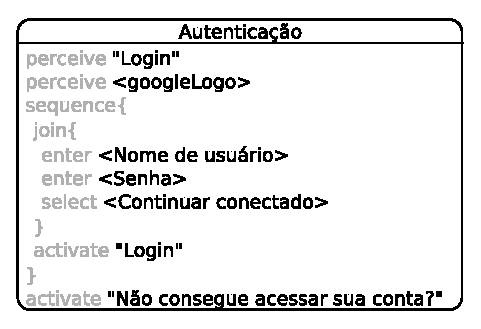
\includegraphics[scale=1.000]{images/login-web-is.eps}
%      \label{fig:espaco-de-interacao-a}
%    } 
%    \quad
%    \subfigure[Formulário web]{
%      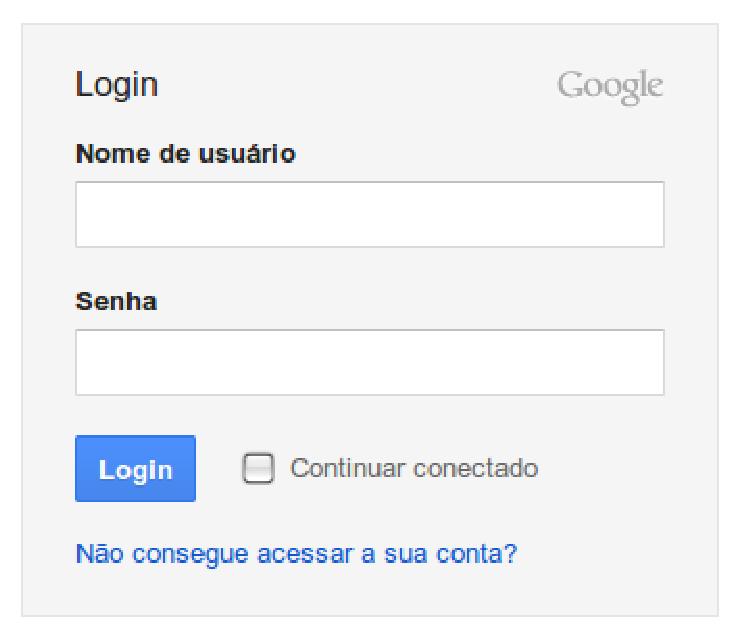
\includegraphics[scale=0.500]{images/login-web.eps}
%      \label{fig:espaco-de-interacao-b}
%    }
%
%    \caption{Exemplo  de  um  espaço  de  interação  representando  um
%      formulário web.}
%
%    \label{fig:espaco-de-interacao}
%  \end{center}
%\end{figure}
%
%O  espaço   de  interação  da  figura~\ref{fig:espaco-de-interacao-a},
%expressa a  seguinte semântica  ou intenção comunicativa  do designer:
%``aqui/agora você pode  efetuar o {\em Login} na  aplicação, para isso
%você deverá primeiro fornecer pelo menos as informações para {\em Nome
%  do usuário} e {\em Senha},  depois ativar o {\em Login} para acionar
%a  função da  aplicação  correspondente.  Se  houver  interesse que  o
%sistema  mantenha  suas  informações  para  uso  em  sessões  futuras,
%selecione  {\em Continuar  conectado},  antes de  ativar {\em  Login}.
%Caso tenha problemas  na autenticação, ative o link  {\em Não consegue
%  acessar sua conta?}  para mais informações''. Dito de outra forma, o
%que  ele quer  que seja  comunicado ao  usuário, através  da interface
%naquele ponto do processo de interação.  Em resumo, {\em o que} e {\em
%  como} o usuário deve agir para usufruir dessa funcionalidade.
%
%Concretamente,  tem-se  como  exemplo  uma janela,  em  uma  interface
%gráfica, ou um formulário, em uma página Web, onde existem vários {\em
%  widgets}  usados pelo  usuário para  entrar com  os dados,  ativar a
%execução da funcionalidade  correspondente e visualizar os resultados.
%Como  visto, os  {\em  widgets}  para entrada  de  dados, ativação  de
%processos e  visualização dos resultados são  representados pelas {\em
%  interações  básicas}.  Na  figura~\ref{fig:espaco-de-interacao-b}, é
%possível  perceber  um   formulário  associado  a  uma  funcionalidade
%específica oferecida pelo sistema, com seus respectivos {\em widgets},
%para o usuário comandar aquela funcionalidade.
%
%Como já  dito, em geral,  um espaço de  interação está ligado,  a pelo
%menos,  uma   função  da  aplicação,   que  deve  ser   sua  principal
%funcionalidade.  Isso pode confundir o leitor levando-o a imaginar que
%um  espaço  de interação  permite  ao  usuário  comandar mais  de  uma
%funcionalidade da aplicação. Em termos de objetividade, não é isso que
%ocorre.   Contudo,  em  muitas  situações, a  interface  realiza,  por
%exemplo, diversas  consultas ao sistema,  principalmente para produzir
%listas  de  faixa de  valores  a serem  usados  pelo  usuário para  se
%produzir as informações necessárias  à execução da função da aplicação
%principal.
%
%Para exemplificar  tal situação, tem-se  uma interface onde  o usuário
%deve  selecionar uma cidade  para indicar  seu endereço,  porém, antes
%deve selecionar o  estado, fazendo com que a  ativação de uma consulta
%seja realizada pelo sistema e  a lista de cidades seja disponibilizada
%na  interface para posterior  seleção do  usuário. Outro  exemplo, bem
%comum atualmente,  são as  aplicações Web, com  suporte a  campos {\em
%  autocomplete}, que  realizam consultas  ao sistema a  cada caractere
%digitado naquele  campo e  produzem uma lista  de sugestão  de valores
%para que o usuário possa selecionar aquele que lhe interessar, sem ter
%que completar a digitação.
%
%Para  mostrar como  o designer  pode usar  \aladim\ para  modelar essa
%situação,      pode      se       observar      o      exemplo      da
%figura~\ref{fig:IncluirCliente}.   Como as  transições  são provocadas
%sempre  por uma  interação  básica  dentro do  espaço  de interação  é
%possível perceber que, quando a interação básica ``select <estado>'' é
%executada,  ocorre a  transição  de ativação  da  função da  aplicação
%``consultaCidades''. Após a execução  do processo, sua transição é uma
%reação de  sucesso, com  uma lista de  cidades associada  à informação
%<cidade>,  para  o espaço  de  interação,  no  qual o  usuário  poderá
%continuar  no processo  de interação  e selecionar  uma  cidade dentre
%aquelas  listadas  para  o  estado  selecionado  na  interação  básica
%anterior.
%
%\figura{Espaço de interação com múltiplas funções da aplicação.}
%       {fig:IncluirCliente}
%       {incluir-cliente.eps}
%       {0.950}
%       {0}
%
%É  importante ressaltar que  numa perspectiva  comunicativa e  com uma
%preocupação  na   escolha  de  signos   que  mantenham  o   mínimo  de
%consistência  dentro do modelo,  sugere-se que  a principal  função da
%aplicação que estabelece a motivação de se interagir com aquele espaço
%de interação, apresente-se estritamente relacionada à identificação do
%espaço  de  interação.   Essa   preocupação  acontece  no  exemplo  da
%figura~\ref{fig:IncluirCliente},  onde  o  espaço  de  interação  está
%associada   às    funções   de   aplicação    ``consultarCidades''   e
%``incluirCliente''. Nela  é possível  observar que essa  última função
%possui a mesma identificação que  o espaço de interação.  Isso permite
%que não se levante  dúvida sobre qual é a função principal  e qual é a
%secundária,  usada  para auxiliar  o  usuário  no processo  interativo
%necessário para comandar a função principal.
%
%A modelagem da  interação do usuário com o  sistema, usando \aladim, é
%guiado  pelo diagrama de  casos de  uso, o  que torna  possível ter-se
%apenas  um modelo  para  uma  aplicação modesta  com  poucos casos  de
%uso. Contudo,  é comum que se  tenha aplicações com  elevado número de
%casos  de  uso,  de  maneira  que  produzir e  ler  apenas  um  modelo
%\aladim\ para todos os casos de uso pode ser frustante.
%
%Diante disso, é  possível construir um modelo \aladim\  para cada caso
%de  uso  ou  até  um  conjunto  deles.   Contudo,  para  se  manter  a
%consistência  do modelo  como  um  todo, é  necessário  se garantir  a
%rastreabilidade das transições  possíveis entre os respectivos espaços
%de interação,  definidos ao longo dos  vários modelos de  cada caso de
%uso. Portanto, ao  se modelar a interação para  um determinado caso de
%uso, é  possível identificar a  necessidade de referenciar  espaços de
%interações presentes  ou definidos em  modelos de interação  de outros
%casos de uso.
%
%Com    o     exemplo    dessa    situação     pode-se    observar    a
%figura~\ref{fig:ReferenceInteractionSpace},  cujo modelo  de interação
%para um caso de uso  de ``Escrever mensagem'', apresenta a intenção do
%designer em comunicar:  (a) que o processo de  interação inicia-se com
%uma transição vinda de um  espaço de interação definido noutro modelo,
%de outro  caso de  uso e  que foi provocada  por uma  interação básica
%identificada (naquele espaço de interação) por ``escrever''; (b) que a
%interação usuário-sistema  se dará através  de um espaço  de interação
%para  o  usuário  produzir  as informações  necessárias,  ativação  da
%funcionalidade  correspondente,  incluindo  situações  de  exceção  na
%execução e a  desistência por parte do usuário; (c)  que no sucesso do
%envio da mensagem, ou na  desistência do usuário de postar a mensagem,
%o  processo de interação  se encerrará  com as  respectivas transições
%para o espaço de interação ``Examinar mensagens''.
%
%\figura{Exemplo de referência para um espaço de interação.}
%       {fig:ReferenceInteractionSpace}
%       {ReferencelInteractionSpace.eps}
%       {0.850}
%       {0}
%
%Isso permite dizer que, apesar da fragmentação do modelo de interação,
%é  possível  se  manter   a  rastreabilidade  sobre  os  artefatos,  e
%principalmente, a consistência na  representação do processo global de
%interação.  Isto  é, mesmo modelando a  interação para um  caso de uso
%específico,  busca-se facilitar a  identificação da  seguinte situação
%dentro do  processo de interação: ``de  onde o usuário  veio, antes de
%chegar naquele ponto do processo de  interação, o que ele pode fazer e
%como fazê-lo e para onde ele irá a partir daquele ponto''.
%
%Na   figura~\ref{fig:ReferenceInteractionSpace},    no   contexto   de
%``Escrever mensagem'', é possível  reconhecer que o fluxo de interação
%veio do  espaço de interação ``Examinar  mensagens'', detalhado noutro
%contexto,  e  irá voltar  para  o mesmo,  logo  após  a execução,  com
%sucesso,   da  função   de  aplicação   ``enviarMensagem'',   ou  pela
%desistência do envio por parte do usuário.
%
%Existem ainda situações  em que a aplicação sendo  modelada permite ou
%exige  que o  usuário interaja  com  outra aplicação.   Nesse caso,  o
%processo  de interação  irá ocorrer  dentro dos  espaços  de interação
%daquela  aplicação, que  por  sua  vez não  estão  sendo modelados  e,
%portanto, são desconhecidos.  Assim,  o processo de interação modelado
%irá transitar  para um espaço de interação  especial, representado por
%um  retângulo  de  cantos  arredondados com  apenas  um  compartimento
%contendo o nome da aplicação  e terá suas bordas desenhadas com linhas
%tracejadas,               como               ilustrado              na
%figura~\ref{fig:ExternalInteractionSpace}.
%
%\figura{Exemplo de um espaço de interação externo à aplicação.}
%       {fig:ExternalInteractionSpace}
%       {ExternalInteractionSpace.eps}
%       {0.750}
%       {0}
%
%%=====================================================================
%\subsection{Função da aplicação}
%\label{applicationFunctions}
%%=====================================================================
%
%Uma {\em função da aplicação} é usada para representar onde e quando o
%sistema   irá  atuar  no   processo  de   interação,  especificamente,
%executando um  processo que realiza  alguma das regras (ou  lógica) de
%negócio da aplicação, ou seja,  os serviços que a aplicação oferece ao
%usuário  para ele  realizar  suas tarefas.   Uma  função da  aplicação
%poderá produzir novas informações  e retornar aos espaços de interação
%para informar o usuário dos resultados do processo.  São representadas
%por retângulos  com dois compartimentos,  sendo o primeiro  usado para
%sua identificação e o  segundo reservado para alguma possível expansão
%futura.     Uma    função   da    aplicação    é   exemplificada    na
%figura~\ref{fig:ApplicationFunction}.
%
%\figura{Exemplo de função da aplicação.}
%       {fig:ApplicationFunction}
%       {application-function.eps}
%       {0.750}
%       {0}
%
%Como todo  processo computacional, as funções da  aplicação consomem e
%produzem informações  quando são  executadas pelo sistema,  contudo, a
%especificação das  funcionalidades da aplicação,  como se faz  na \es,
%não  é  endereçada  em  \aladim\.   O designer,  como  já  dito,  está
%preocupado em  modelar {\em o que}  o usuário pode fazer  e {\em como}
%ele deve agir para  usufruir do sistema e não em modelar  {em o que} o
%sistema faz e {\em como} se comporta para atender ao usuário.
%
%Dessa forma, alguns desses aspectos sobre a função da aplicação já são
%cobertos  no modelo,  sem os  rigores da  \es, através  das interações
%básicas  postas  nos respectivos  espaços  de  interação associados  à
%função da aplicação; de maneira  que as informações que esta necessita
%e  produz  sejam,  respectivamente,  fornecidas e  percebidas,  nesses
%espaços        de       interação,       vide        exemplos       da
%figuras~\ref{fig:interaction-space-all}.    Além   disso,  mesmo   não
%endereçando  seus mecanismos  de  controle interno  como suspensão  ou
%interrupção,  por exemplo, \aladim\  permite modelar  o que  o usuário
%precisa  fazer  para  controlar  a  execução  também  nos  espaços  de
%interação, através  das respectivas interações básicas,  como pode ser
%observado no exemplo da figura~\ref{fig:copy-files}.
%
%Também  é  importante  destacar   que  as  funções  da  aplicação  são
%abstrações  para   as  funcionalidades  oferecidas   pelo  sistema,  e
%consequente,  também estão  associadas  aos casos  de uso,  levantados
%durante a análise dos requisitos da aplicação. Portanto, se o designer
%estiver modelando  a interação num  único modelo diagrama,  ele deverá
%possuir no mínimo uma função de aplicação para cada caso de uso.
%
%%=====================================================================
%\subsection{Transições}
%\label{transitions}
%%=====================================================================
%
%Para comunicar onde e quando se darão as mudanças de quem irá atuar no
%processo  de   interação,  deve-se  usar  uma   {\em  transição}.   As
%transições de um  espaço de interação para outro  podem ser disparadas
%por  qualquer  interação  básica  dentro  do espaço  de  interação  de
%origem. Cada  uma delas deve ser  representada por uma  linha sólida e
%possuir,  como rótulo,  o nome  da  interação básica  que a  disparou.
%Outra possibilidade é  por inatividade do usuário, nesse  caso, a seta
%deverá possuir rótulo com um valor temporal (ex.  50s, 3min) indicando
%que  após aquele  tempo de  inatividade  do usuário,  a transição  irá
%ocorrer.
%
%Existem duas  situações de transição  entre espaços de  interação.  Na
%primeira  não há  demanda  por funcionalidade  da  aplicação, isto  é,
%tem-se  apenas uma  {\em  navegação}.  Nesse caso  não  há mudança  da
%atuação do usuário para o  sistema, apenas que o usuário poderá/deverá
%continuar atuando em outro espaço de interação.  Essa situação é comum
%em espaços de interação que concentram chamadas a outros espaços, como
%janela com menus, por exemplo. A segunda é quando a transição demandar
%a execução de uma função da aplicação, sendo tratada de duas maneiras.
%
%Quando partir do espaço de  interação para a função da aplicação, onde
%é   considerada  uma   {\em  ação}   do  usuário   solicitando  alguma
%funcionalidade do sistema, deve ser representada por uma linha sólida.
%Quando  a transição  parte da  função da  aplicação para  o  espaço de
%interação,  é  considerada uma  {\em  reação}  do  sistema à  ação  do
%usuário, podendo ser representada de duas formas: (a) se a execução da
%função  da aplicação  terminar normalmente  será representada  por uma
%linha sólida, cujo rótulo  poderá ser alguma informação retornada pela
%função ou  uma mensagem explícita do  designer para o  usuário; (b) no
%caso da execução terminar de maneira anormal, a linha será tracejada e
%seu rótulo poderá ser alguma  indicação do motivo da falha, através de
%uma mensagem  explícita do designer e/ou alguma  informação do domínio
%ou      da      aplicação,      como     podemos      observar      na
%figura~\ref{fig:interaction-space-all}.
%
%\figura{Exemplo de um espaço de interação e função da aplicação.}
%       {fig:interaction-space-all}
%       {calculating-value-all.eps}
%       {0.700}
%       {0}
%
%As transições são usadas para indicar uma mudança do fluxo de ações do
%usuário para  o fluxo  de reações do  sistema.  Ainda  nesse contexto,
%existem  situações especiais em  que o  usuário poderá  realizar novas
%interações  básicas enquanto aguarda  uma reação  do sistema  para uma
%ação já  executada.  Nesse caso, o  espaço de interação  deve estar em
%``sincronismo''   com  a   função  da   aplicação.   Esta   ligação  é
%representada  por  setas  de   duplo  sentido.   Elas  são  destinadas
%exclusivamente para  representar uma ligação síncrona  entre um espaço
%de  interação e  uma  função da  aplicação.   Isto é,  mesmo quando  o
%processo  está em execução,  o usuário  poderá observar  seu progresso
%e/ou  intervir sobre o  mesmo.  Nesse  caso, a  seta não  deve possuir
%rótulo, como exemplificado na figura \ref{fig:copy-files}, onde depois
%de ter iniciado  o processo em {\em Copiar  arquivos}, o usuário, além
%de acompanhar o seu progresso, poderá suspender, reiniciar ou cancelar
%o processo em {\em Copiando arquivos}.
%
%\figura{Modelo para um cenário para cópia de arquivos.}
%       {fig:copy-files}
%       {copy-files.eps}
%       {0.650}
%       {0}
%
%%=====================================================================
%\section{Construindo um modelo completo}
%\label{aladimExamples}
%%=====================================================================
%
%Nesta  seção, é  apresentado um  exemplo de  como se  construir modelo
%completo, mesmo  que de tamanho limitado, usando  a linguagem \aladim,
%mostrando  principalmente  como   identificar  as  porções  do  modelo
%associadas aos casos  de uso da aplicação. Nesse  exemplo, trata-se de
%um modesto  sistema de correio  eletrônico, com um número  restrito de
%funcionalidades,  cujos requisitos  são especificados  no  diagrama de
%casos  de  uso  apresentado na  figura~\ref{fig:Email:System:Usecase},
%construída   usando    uma   versão   grátis    da   ferramenta   {\em
%  astah}\footnote{http://astah.net/editions/uml}.     O    modelo   de
%interação  correspondente,  na  linguagem  \aladim, é  apresentado  no
%diagrama da figura~\ref{fig:Email:System:Aladim}.
%
%\figura{Diagrama de casos de uso para um sistema 
%  de correio eletrônico.}
%       {fig:Email:System:Usecase}
%       {email-system-uc.eps}
%       {0.650}
%       {0}
%
%Na    figura~\ref{fig:Email:System:Aladim},    pode-se   observar    a
%correspondência  unitária  entre os  casos  de  uso  e os  espaços  de
%interação.  Isso  está ligado  ao fato de  um espaço de  interação ser
%usado para comunicar todo o conjunto de interações básicas necessárias
%para se usufruir  de determinada funcionalidade da aplicação,  o que é
%identificado   como  um  requisito   funcional  e   representado  pelo
%respectivo  caso  de uso.   Outra  importante  observação  é quanto  à
%visualização  dos anexos das  mensagens, que  não será  realizada pela
%própria  aplicação e sim  pelo visualizador  de arquivos,  definido no
%sistema operacional,  o que foi  modelado como uma referência  para um
%espaço de interação definido numa aplicação externa.
%
%\figura{Modelo \aladim\ correspondente ao diagrama de 
%  casos de uso da figura~\ref{fig:Email:System:Usecase}.}
%       {fig:Email:System:Aladim}
%       {email-system.eps}
%       {0.525}
%       {-90}
%
%A  figura~\ref{fig:Email:System:Aladim}, traz  um modelo  de interação
%para um sistema simples  de correio eletrônico, cujos requisitos estão
%especificados     no     diagrama     de     caso    de     uso     da
%figura~\ref{fig:Email:System:Usecase}.   Sendo que  para cada  caso de
%uso,  com  duas  exceções,  foi  modelado um  espaço  de  interação  e
%associado  a ele  uma  função da  aplicação  representando o  processo
%computacional responsável pela realização do caso de uso.
%
%A primeira  exceção foi do caso  de uso {\em Efetuar  logout}, que não
%precisou  de um  espaço de  interação para  isso, bastando  apenas uma
%interação básica  no espaço de  interação {\em Examinar  mensagens}. A
%outra  exceção foi  do caso  de uso  {\em Visualizar  anexos},  que na
%verdade, foi modelado com uma referência para uma aplicação externa ao
%sistema sendo desenvolvido.
%
%%=====================================================================
%\section{Considerações sobre o capítulo}
%\label{aladimSynthesis}
%%=====================================================================
%
%\aladim\  foi  concebida para  auxiliar  o  designer,  não só  na  sua
%comunicação com o usuário por meio da interface, mas também com aquele
%que  antecede  e  atua  como  um tradutor  para  essa  comunicação,  o
%desenvolvedor. Dessa forma, neste trabalho, o design da interação como
%proposto no ciclo  de vida da figura~\ref{fig:Design:Lifecycle:Model},
%considera  que   o  primeiro  estágio  desse   ciclo,  que  compreende
%principalmente os requisitos, será finalizado com um diagrama de casos
%de uso.   A partir desse diagrama é  que o designer irá  lançar mão de
%\aladim\ para  modelar o processo  de interação necessário para  que o
%usuário possa  fazer uso das funcionalidades  oferecidas pelo sistema,
%representadas  no  diagrama  de   casos  de  uso  como  requisitos  da
%aplicação.
%
%Como já visto, \aladim\ se baseia  na \se\ para auxiliar o designer no
%processo comunicativo com o usuário.   Isso é possível através de seus
%elementos,  conceitualmente  definidos de  maneira  que seja  possível
%modelar  e  refletir  sobre  a  interação, estruturando  o  modelo  de
%interação  como  uma  mensagem   interativa  que  comunica  a  própria
%interação.  Dessa forma, a estrutura da mensagem interativa é composta
%por  {\em espaços  de  interação},  que comandam  a  execução de  {\em
%  funções  da  aplicação}.   Os  comandos  ocorrem  através  das  {\em
%  interações básicas},  que permitirão ao usuário  produzir e consumir
%as informações  necessárias à  execução da funcionalidade  em questão,
%bem como acionar sua execução.   Cada espaço de interação poderá estar
%organizado  por meio  dos {\em  operadores}, que  permitem estabelecer
%vários tipos  de relacionamentos entre as interações  básicas; o fluxo
%de interação entre os vários espaços de interação, bem como destes com
%as funções de aplicação, é comunicado através das {\em transições}.
%
%Como demostrado na definição dos elementos da linguagem, o embasamento
%na \se\ se fez necessário pela preocupação com o aspecto comunicativo,
%tanto  da linguagem  em  si,  quanto do  produto  final resultante,  o
%sistema  interativo. Cada  elemento de  \aladim\ possui  esse aspecto,
%isto  é,  se  constitui  como  um  signo que  irá  compor  a  mensagem
%estruturada  do  design  sobre  o  diálogo entre  usuário  e  sistema,
%comunicando quais  as ações que  o usuário pode/deve executar  e quais
%reações esperar do sistema, em resumo, o modelo de interação.
%
%%%% Local Variables: 
%%%% mode: latex
%%%% TeX-master: "main"
%%%% End: 
